\chapter{Experimental Results}
\label{chap:results}

We conducted an experimental evaluation of our algorithms, with two major driving goals in mind: study the behavior of the algorithms presented in this thesis and compare it with that of state of art algorithm \ref{algo:brande} in terms of execution time.

\section{Implementation and environment}
We implemented our algorithms and the one presented in algorithm \ref{algo:brande} on IITM's Libra cluster node which has 74GB RAM size and using 18GB as maximum heap space. 

\vspace{-1.5em}
\section{Results}
We have compared our algorithm with Brandes' algorithm and we found that there is huge reduction in execution time.
\vspace{-1.0em}
\subsection{Results for Algorithm on Tree}
The trees used for the experimental purposes are synthetic trees made through random functions.
The synthetic trees which were developed used a random function which generated a random number and that generated number was used as a degree for that particular vertex. And correspondingly new edges were added from that vertex. It was made sure that, the generated graph is a tree or a forest and does not have any cycle

As we can see in table \ref{tab:res1}, that as per increase in the number of vertices of the tree, the time taken by Brandes' algorithm increases to a large extent as compared to proposed algorithm. This proves the basis which we stated to reduction in  time complexity for computing betweenness centrality for trees. As we can see that in Figure \ref{fig:res1}, the speed up increases linearly with respect to number of vertices.

\begin{table}[h!]
\centering
\begin{tabular}{|c|c|c|}
\hline
No.of vertices & Proposed algorithm on tree & Brandes' algorithm \\
\hline
 & Time in sec & Time in sec\\ 
\hline
2000 & 0.10 & 76.7 \\ 
\hline
4000 & 0.11 & 387.3 \\ 
\hline
6000 & 0.12 & 1093.4 \\ 
\hline
8000 & 0.13 & 2005.5 \\ 
\hline
\end{tabular}
\caption{Comparison of Brandes' algorithm with our algorithm}
\label{tab:res1}
\end{table}




\begin{figure}[h]
%\begin{center}

\subfigure[]{
        %\centering
        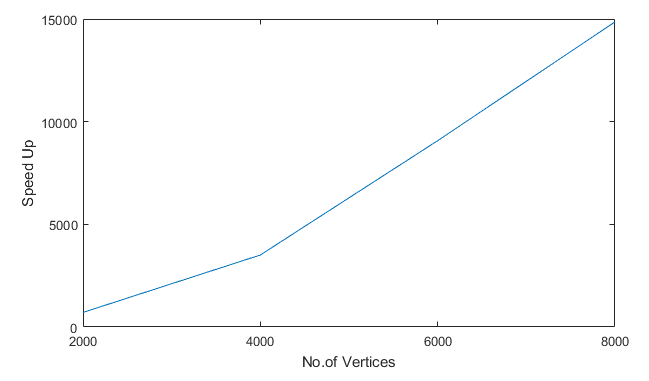
\includegraphics[width=8cm]{images/speed_up.png}
        %\subcaption{Experimental setup}
        \label{fig:res1}
}
\subfigure[]{
        %\centering
        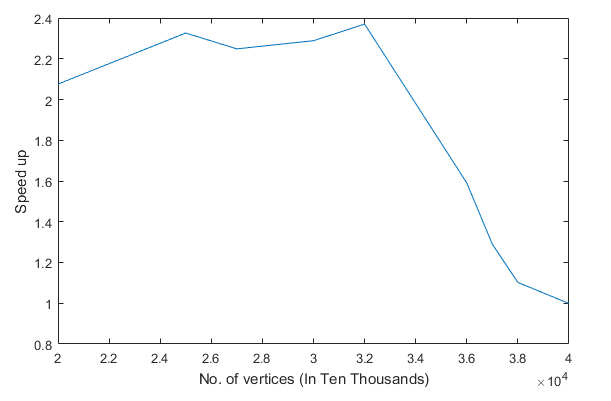
\includegraphics[width=8cm]{images/speed_up_2.png}
        %\caption{Image taken by two photon microsope}
        \label{fig:res2}
}
\caption{Speed Up of our algorithm (a) Tree (b) DAG}
\label{fig:tree1}
%\end{center}
\end{figure}


\subsection{Results for Algorithm on DAGs}
The DAGs used for the experimental purposes are synthetic DAGs made through random functions.
The synthetic DAGs which were developed used a random function which generated a random number and that generated number was used as a degree for that particular vertex $v$. And correspondingly new edges were added from that vertex $v$ to a vertex $u$ randomly chosen within a range with a higher value that vertex $v$. It was made sure that, the generated graph is a DAG does not have any cycle.

As we can see in table \ref{tab:res2}, that as per increase in the number of vertices of the tree, the time taken by Brandes' algorithm increases and the time required by our algorithm increases to a large extent but still is less than Brandes' algorithm.
In Figure \ref{fig:res2}, the speed up achieved is around 2 and then it decreases as the number of vertices increases and becomes 1.
As the number of vertices increases, not much performance gain is achieved because we use huge memory and once the memory is used up, the program takes huge amount of time swapping the memory in and out of RAM. Also for more higher number of vertices, our algorithm doesn't work the heap space provided.
Hence we can conclude that, if given enough memory to compute betweenness centrality, our proposed algorithm beats the Brandes' algorithm.


\begin{table}[h!]
\centering
\begin{tabular}{|c|c|c|c|}
\hline
No.of vertices & No.of edges & Proposed algorithm on DAG & Brandes' algorithm \\
\hline
 & & Time in sec & Time in sec\\ 
\hline
20000 & 91207 & 57.9 & 120.2 \\ 
\hline
25000 & 111852 & 88.9 & 206.8 \\ 
\hline
27000 & 121079 & 109.5 & 246.4 \\ 
\hline
30000 & 134769 & 124.9 & 285.9 \\ 
\hline
32000 & 144339 & 141.9 & 336.4 \\ 
\hline
36000 & 163172 & 246.0 & 391.1 \\ 
\hline
37000 & 165877 & 333.3 & 429.9 \\ 
\hline
38000 & 170896 & 435.1 & 479.5 \\ 
\hline
40000 & 179765 & 625.0 & 626.2 \\ 
\hline
\end{tabular}
\caption{Comparison of Brandes' algorithm with our algorithm}
\label{tab:res2}
\end{table}